\chapter{Threats}
\section{Threats to the birds}
 Three major threats  to the birds were identified.
\begin{enumerate}
    \item Destruction of habitats
    \item Water pollution in Bolgoda lake around the boat yard.
    \item Spreading of invasive alien plant species.
\end{enumerate}
\begin{figure}[!htpb]
    \centering
    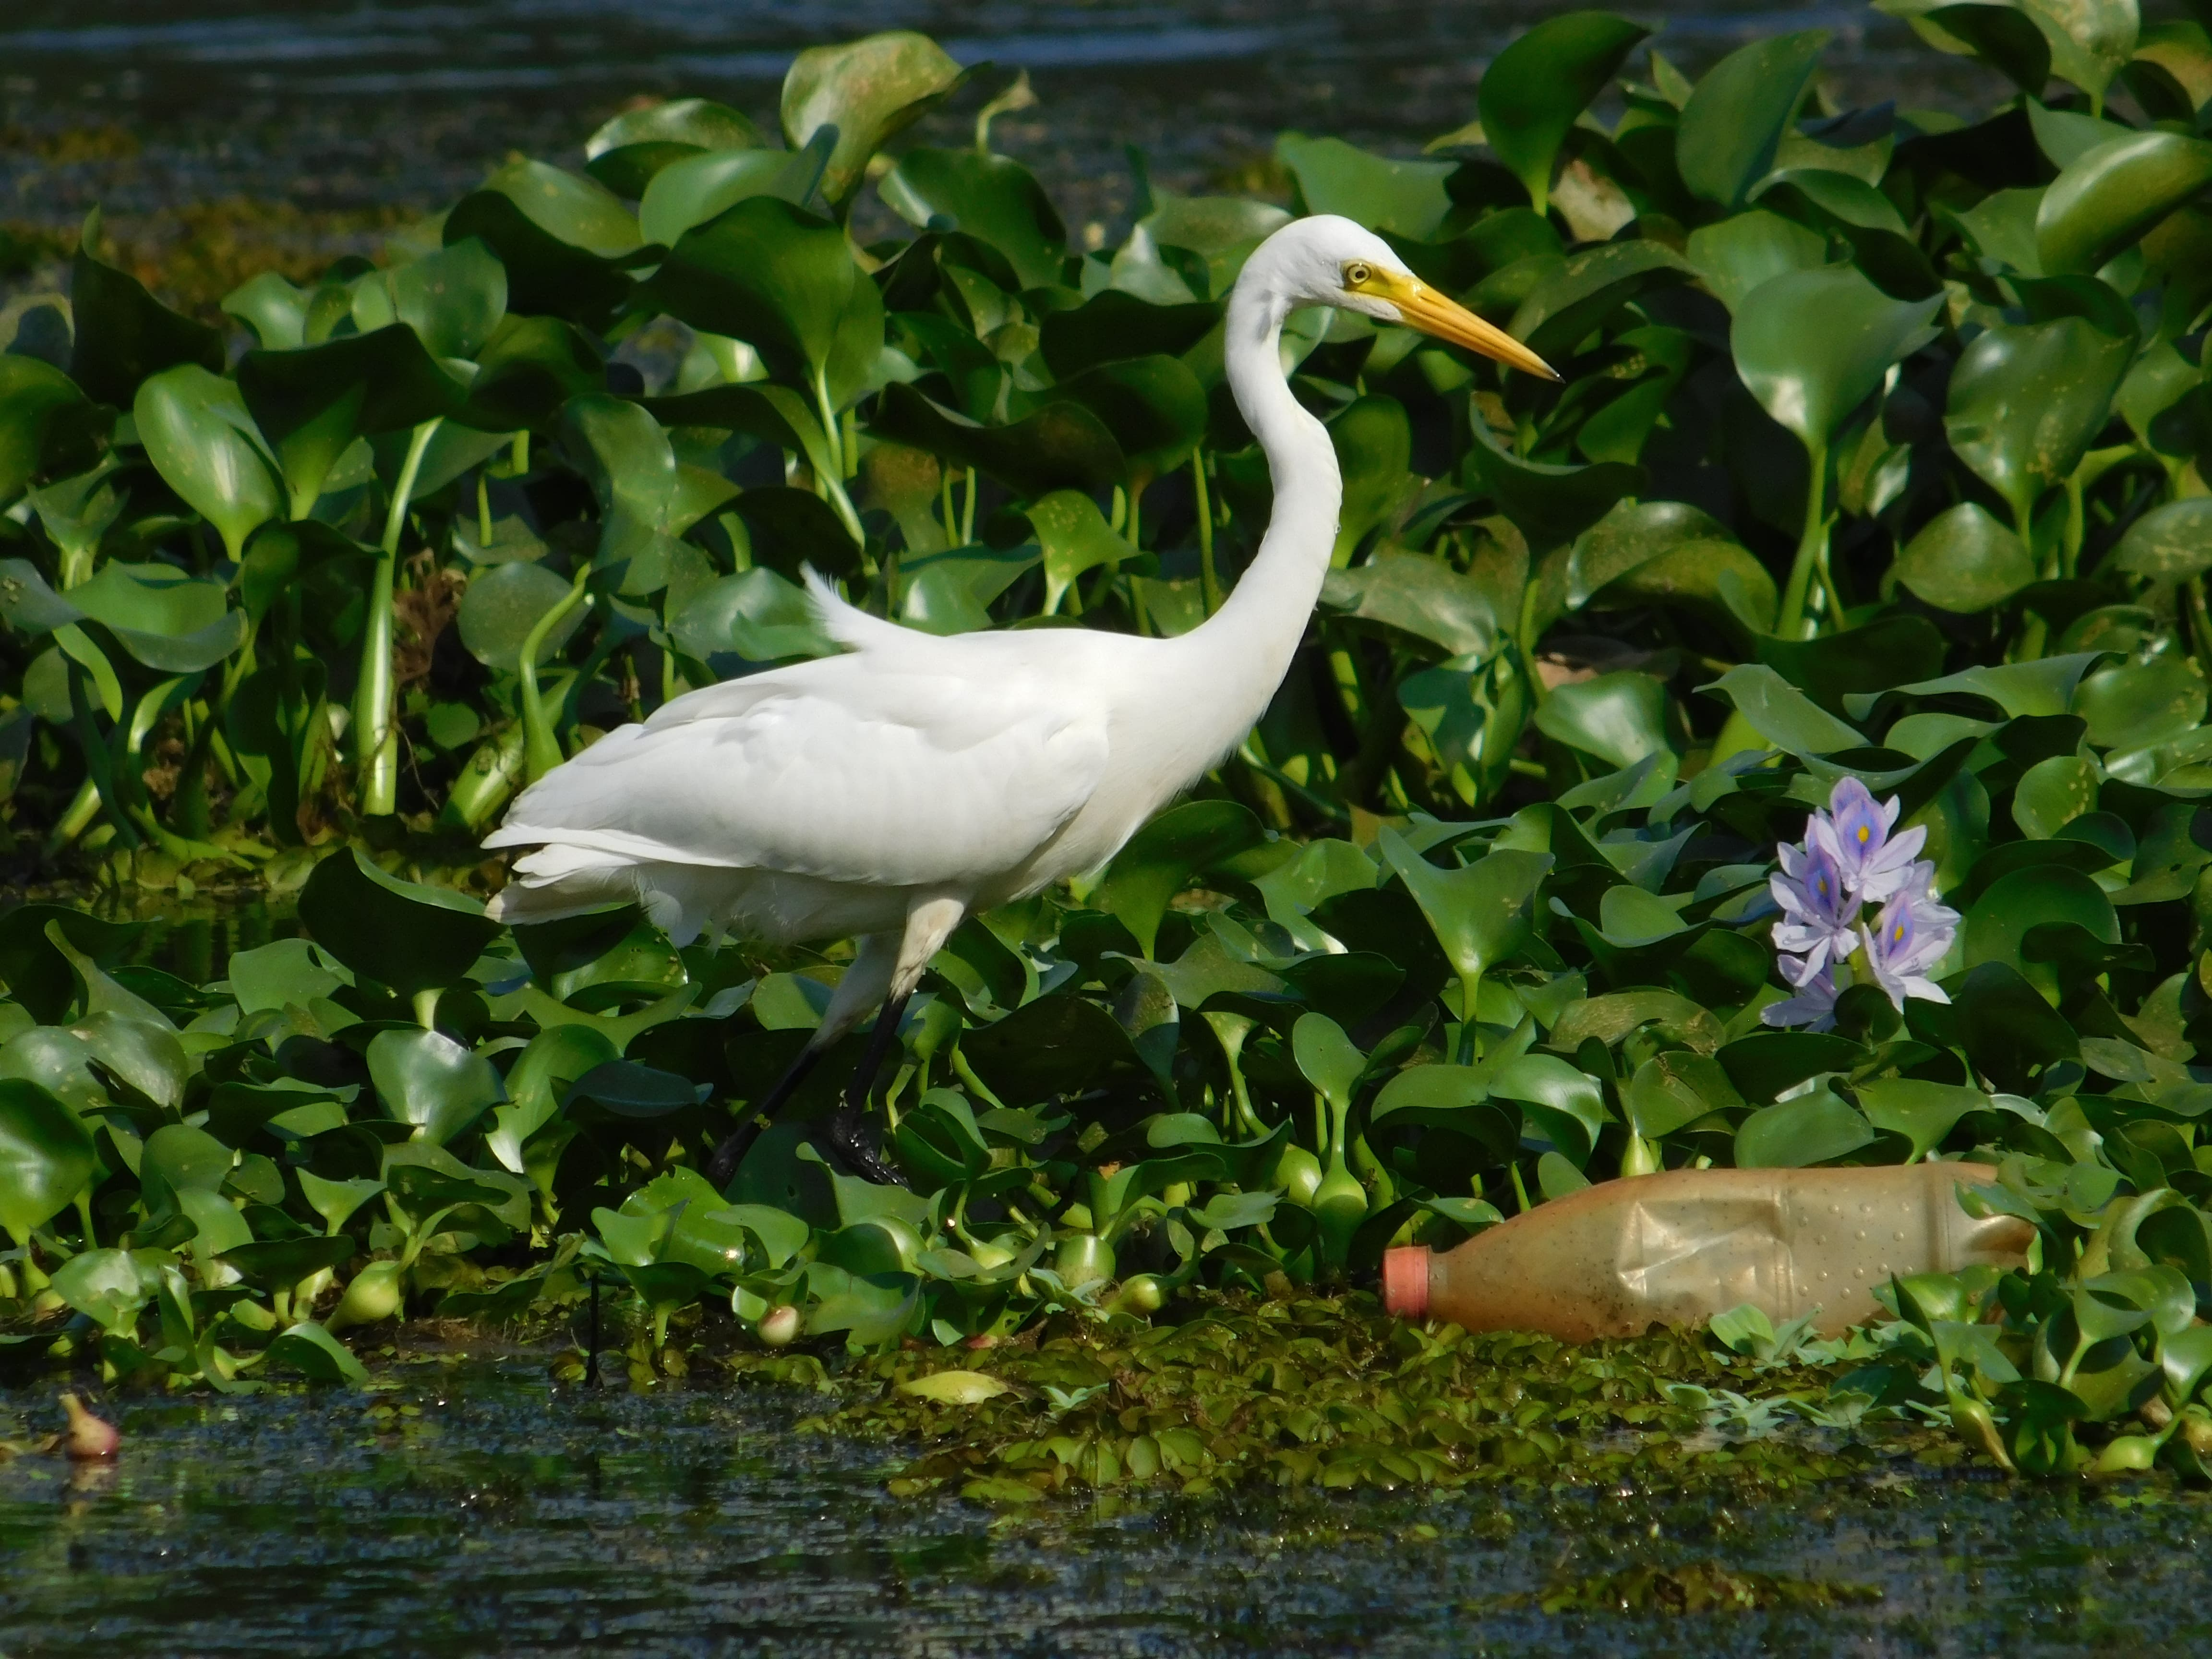
\includegraphics[width=0.955\textwidth]{Figures/threats.jpg}
    \caption[]{An Intermediate Egret hunting in the Boat Yard, surrounded by a dumped plastic bottle, Common water hyacinth,Water lettuce and Salvinia.}
    \label{fig:figure-01}
\end{figure}
\subsection{Habitat Loss}
The natural habitats of birds near the university are under constant threat and diminishing due to urban development. The limited available land faces high demand for various purposes, such as construction, leading to significant and impacting destruction. A recent example occurred on February 5th, 2024, when a tree between A-hostel and the main building of the Department of Civil Engineering was cut down, containing a nest of spotted doves with chicks.
    \begin{figure}[!htpb]
        \centering
        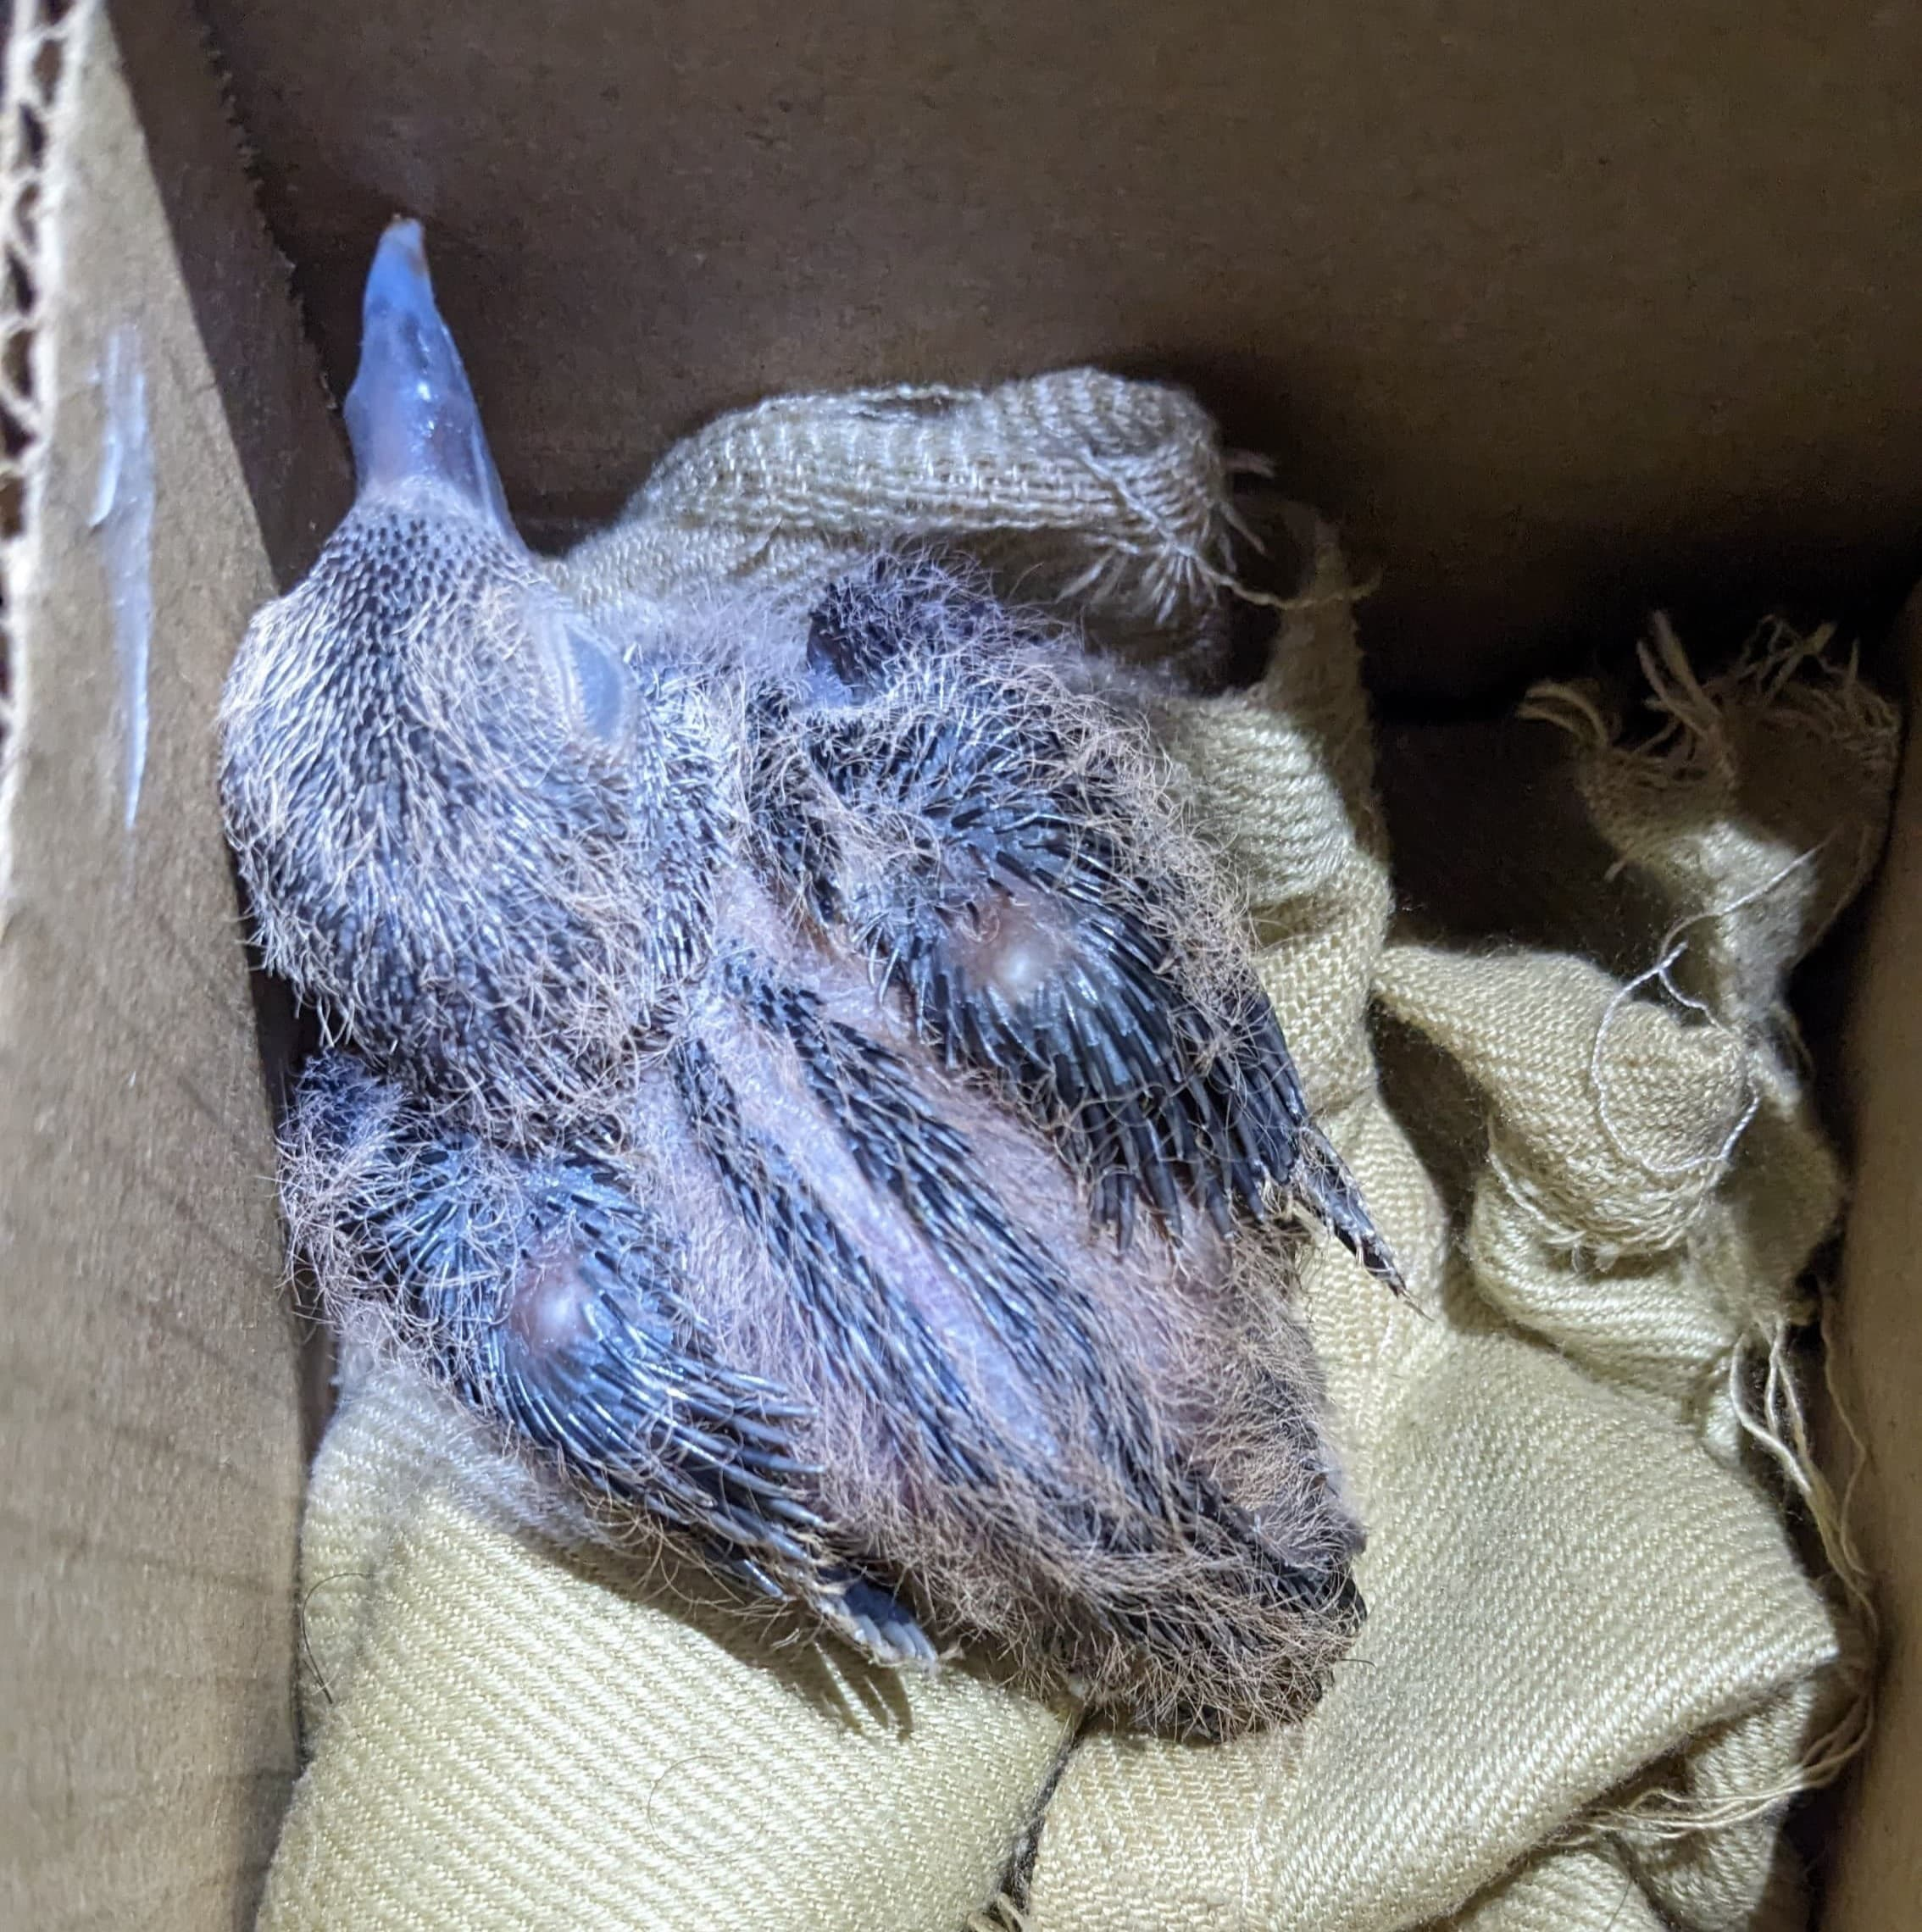
\includegraphics[width=\linewidth]{Figures/spotted-dove-chick.jpg}
        \caption[]{A Spotted Dove chick rescued from the tree that was cut down.}
        \label{fig:figure-01}
    \end{figure}

\subsection{Water Pollution}
Water pollution in the Bolgoda lake area around the Boat yard is from the indiscriminate disposal of waste and the release of effluents. This environmental degradation has adverse effects on both water quality and the diverse aquatic species that serve as prey for numerous birds, including various fish species and crustaceans.
\subsection{Invasive Alien Plants}
Furthermore, the rapid proliferation of following invasive alien species poses an ongoing threat to avian populations.

\begin{itemize}
\item Common Water Hyacinth (\textit{Eichhornia crassipes})
\item Water Lettuce (\textit{Pistia stratiotes})
\item Hydrilla (\textit{Hydrilla verticillate})
\item Salvinia (\textit{Salvinia molesta})
\end{itemize}
These invasive species not only endanger prey species but also cover the open water surface, hindering hunting opportunities for some bird species, despite potentially serving as floating platforms for some others.
